\chapter{BỘ DỮ LIỆU VÀ THIẾT LẬP THỰC NGHIỆM}
\label{chuong4}
\label{ch:bo_du_lieu_va_thuc_nghiem}

\vspace{-1.5cm} 

\begin{quotation}
    \noindent
    \small\textit{
   Chương này mô tả bộ dữ liệu SHOT và các bộ dữ liệu đánh giá bổ sung, các chỉ số đo lường hiệu quả như Precision, Recall và F1-score, các mô hình cơ sở được so sánh, cùng thiết lập huấn luyện và suy diễn của AutoShot và AutoShotV2. Các bảng kết quả, phân rã và phân tích lỗi được trình bày riêng ở Chương~\ref{ch:ket_qua_thuc_nghiem}.
    }
\end{quotation}
\vspace{1em} % Tạo khoảng cách nhỏ


\section{Bộ dữ liệu SHOT}
SHOT~\cite{zhu2023autoshot} (Short Video Shot Boundary Detection Dataset) là bộ dữ liệu công khai dành cho tác vụ phát hiện ranh giới cảnh quay (shot boundary detection) trong video ngắn. Các nền tảng video ngắn như TikTok hay Instagram Reels đã thay đổi thói quen tiêu thụ nội dung. Nhu cầu phân tích video chính xác về mặt thời gian là cấp thiết. SHOT cung cấp dữ liệu chuẩn cho video có nhịp độ nhanh và nội dung cô đọng.

Phần lớn các bộ dữ liệu phát hiện biên cảnh (SBD) hiện có như BBC Planet Earth hay RAI~\cite{baraldi2015rai} chỉ chứa phim tài liệu hoặc talk show với cảnh quay tĩnh và nhịp độ chậm. Ngay cả bộ dữ liệu lớn ClipShots cũng chủ yếu chứa các video dài (trung bình 237 giây). SHOT ra đời để lấp đầy khoảng trống này với tư cách là bộ dữ liệu công khai đầu tiên dành riêng cho video ngắn, bao gồm 853 video hoàn chỉnh và 11.606 chú thích cảnh quay, mang tính thách thức cao hơn về nhịp độ và hiệu ứng hình ảnh.



\subsection{Chi tiết bộ dữ liệu}
\begin{itemize}
    \item \textbf{Tên bộ dữ liệu:} SHOT (Short Video Shot Boundary Detection Dataset)
    \item \textbf{Quy mô:} 853 video ngắn và 11.606 chú thích ranh giới cảnh quay
    \item \textbf{Tổng số khung hình:} 960.794 khung hình
    \item \textbf{Tập kiểm tra:} 200 video với 2.716 chú thích chất lượng cao; chuyên gia kiểm duyệt hai vòng
    \item \textbf{Nguồn dữ liệu:} Video từ một nền tảng video ngắn phổ biến
    \item \textbf{Quyền riêng tư:} Làm mờ khuôn mặt bằng công cụ phát hiện khuôn mặt
    \item \textbf{Phương pháp gán nhãn:} Dùng hình thu nhỏ $48\times27$ cho mỗi khung hình; số thứ tự khung hình hiển thị thích ứng để giảm công sức kiểm tra
    \end{itemize}



\subsection{Phân tích bộ dữ liệu}
SHOT được phân tích dựa trên các thách thức đặc thù của video ngắn:
\begin{itemize}
    \item \textbf{Chuyển cảnh dần phức tạp (Complex Gradual Transitions):} Kết hợp nhiều hiệu ứng chuyển cảnh chồng chéo thay vì cắt cảnh dứt khoát.
    \item \textbf{Cấu trúc tam phân (Ternary Structure):} Video dọc thường giữ nguyên phần trên và dưới (chứa liên kết/thương hiệu), chỉ thay đổi nội dung ở giữa, gây khó khăn cho việc phát hiện.
    \item \textbf{Cảnh ảo (Virtual Scenes):} Các video game với hiệu ứng hình ảnh phóng đại và biến đổi liên tục.
    
\end{itemize}

\begin{figure}[H]
    \centering
    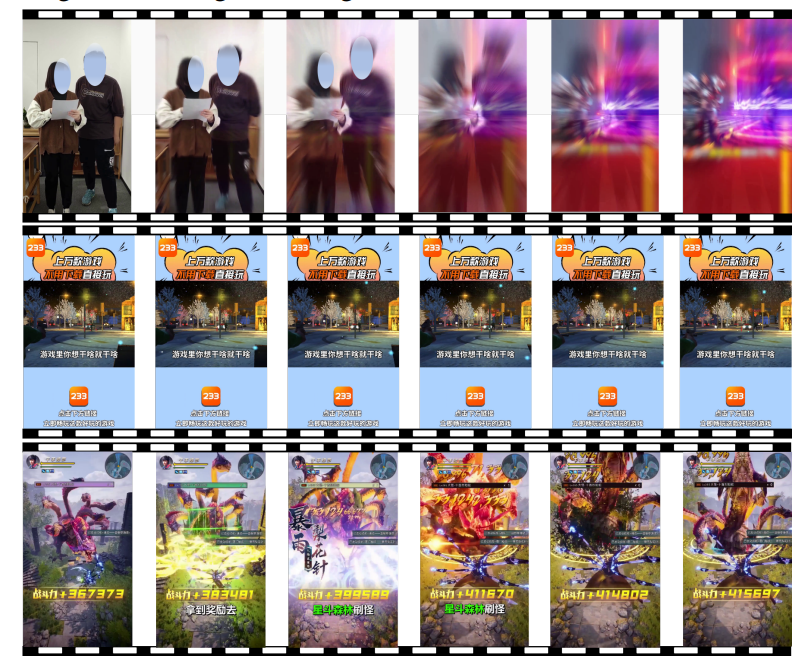
\includegraphics[width=0.8\textwidth]{images/Anh42.png}
    \caption[Minh họa các thách thức đặc thù trong SHOT]{Minh họa các thách thức đặc thù trong SHOT: (Hàng 1) Chuyển cảnh dần phức tạp, (Hàng 2) Cấu trúc tam phân, và (Hàng 3) Cảnh ảo.}
    \label{fig:shot_challenges}
\end{figure}
\FloatBarrier

Sự khác biệt giữa video ngắn và video truyền thống không chỉ nằm ở thời lượng mà còn ở nhịp độ và phong cách hậu kỳ (so sánh chi tiết xem Bảng~\ref{tab:dataset_comparison_detail} ở Mục~\ref{sec:dataset_summary}). Các thống kê chính phản ánh tính chất ngắn và nhanh của bộ dữ liệu:
\begin{itemize}
    \item \textbf{Độ dài trung bình video:} 39.5 giây
    \item \textbf{Độ dài trung bình cảnh:} 2.59 giây
    \item \textbf{Phân bố thời lượng:} 90\% video có độ dài dưới một phút
    \item \textbf{Tốc độ chuyển cảnh:} Hầu hết các cảnh trong tập kiểm tra kéo dài dưới 5 giây; video ngắn có nhịp độ sự kiện nhanh hơn video truyền thống
    \end{itemize}

\begin{figure}[H]
    \centering
    
\includegraphics[width=0.5\textwidth]{images/Anh41.png}
    \caption[Phân bố độ dài video và shot trong SHOT]{Sự phân bố độ dài video (trên) và độ dài shot (dưới). Có thể thấy sự chênh lệch rõ rệt: shot trong SHOT tập trung dày đặc ở vùng dưới 5 giây.}
    \label{fig:shot_distribution}
\end{figure}




\subsection{Ghi chú chuẩn đánh giá từ công trình gốc}
\begin{itemize}
    \item \textbf{Phương pháp:} AutoShot dùng Tìm kiếm kiến trúc nơ-ron (Neural Architecture Search~\cite{elsken2018_nas_survey}) trong không gian gồm 3D ConvNets và Transformers
    \item \textbf{Thiết lập:} Mô hình được huấn luyện trên tập kết hợp SHOT và ClipShots rồi đánh giá trên tập kiểm tra SHOT
    \item \textbf{Kết quả tham chiếu:} Các số liệu so sánh với TransNetV2, AutoShot và các biến thể AutoShotV2 được trình bày ở Chương~\ref{ch:ket_qua_thuc_nghiem}.
    \end{itemize}

\subsection{Tóm tắt}
Với các đặc điểm độc đáo phản ánh đúng thực tế của video ngắn và quy trình gán nhãn chất lượng cao, SHOT không chỉ là một chuẩn mực đánh giá mới mà còn là một tài nguyên quý giá để huấn luyện các mô hình SBD thế hệ tiếp theo. Các kết quả thực nghiệm chi tiết trên SHOT và các bộ dữ liệu bổ sung được trình bày ở Chương~\ref{ch:ket_qua_thuc_nghiem}.

\section{Các bộ dữ liệu đánh giá bổ sung}
Ngoài bộ dữ liệu SHOT dành riêng cho video ngắn, các nghiên cứu về phát hiện ranh giới cảnh quay thường được đánh giá trên nhiều bộ dữ liệu chuẩn khác nhau để kiểm tra khả năng tổng quát hóa. Phần này giới thiệu chi tiết ba bộ dữ liệu phổ biến: BBC Planet Earth, RAI và ClipShots.
Trong phạm vi thực nghiệm của khóa luận này, kết quả định lượng tập trung vào SHOT, BBC và ClipShots; tập RAI chưa được chạy lại do giới hạn tài nguyên tính toán và thời gian.

\subsection{Bộ dữ liệu BBC Planet Earth}
\textbf{BBC Planet Earth}~\cite{baraldi2015rai} gồm 11 tập phim tài liệu thiên nhiên (~50 phút/tập, ~4.900 shot, shot TB 6.57 giây). Nội dung chất lượng cao với camera mượt mà (panning, zooming) và phong cách biên tập nghệ thuật sử dụng nhiều dissolve và fade. Thách thức chính là \textbf{gradual transition} phức tạp khiến ranh giới giữa hai shot không sắc nét như chuyển cảnh đột ngột.

\subsection{Bộ dữ liệu ClipShots}
\textbf{ClipShots}~\cite{tang2018clipshots} là bộ dữ liệu quy mô lớn từ YouTube và Weibo, gồm 4.039 video (TB 237 giây), 128.000+ chuyển cảnh đột ngột và 38.000+ chuyển cảnh dần được dán nhãn thủ công (shot TB 15.34 giây). Nội dung đa dạng (20+ danh mục) từ nghiệp dư đến chuyên nghiệp. Thách thức: thay đổi ánh sáng đột ngột, camera rung, hiệu ứng chuyển cảnh không quy ước (glitch, flash, zoom nhanh) và khoảng cách miền dữ liệu lớn.

\subsection{So sánh tổng hợp các bộ dữ liệu}
\label{sec:dataset_summary}
Bảng \ref{tab:dataset_comparison_detail} tổng hợp các đặc điểm chính của bốn bộ dữ liệu được sử dụng trong đánh giá hiệu năng các mô hình SBD.

\begin{table}[H]
\centering
\small
\begin{tabularx}{\textwidth}{l Y Y Y Y}
\toprule
\textbf{Đặc điểm} & \textbf{BBC} & \textbf{RAI} & \textbf{ClipShots} & \textbf{SHOT} \\
\midrule
Loại nội dung & Phim tài liệu & Talk show & Đa dạng & Video ngắn \\
Số lượng video & 11 & 10 & 4{,}039 & 853 \\
Độ dài TB video (s) & 2{,}945 & 591 & 237 & 39.5 \\
Độ dài TB shot (s) & 6.57 & 5.65 & 15.34 & 2.59 \\
Hard cuts & Nhiều & Nhiều & 128{,}000+ & 8{,}890 \\
Gradual transitions & Rất nhiều & Ít & 38{,}000+ & 2{,}716 \\
Độ khó & Trung bình & Trung bình & Cao & Rất cao \\
Thách thức chính & Gradual transitions & Màu sắc tương đồng & Đa dạng hiệu ứng & Nhịp độ nhanh \\
\bottomrule
\end{tabularx}
\caption{So sánh chi tiết các bộ dữ liệu đánh giá SBD}
\label{tab:dataset_comparison_detail}
\end{table}

Mỗi bộ dữ liệu đại diện cho một khía cạnh khác nhau của bài toán SBD trong thực tế:
\begin{itemize}
    \item \textbf{BBC Planet Earth:} Đánh giá khả năng xử lý chuyển cảnh dần dần trong nội dung chuyên nghiệp.
    \item \textbf{RAI:} Đánh giá khả năng phân biệt shot trong môi trường studio với màu sắc đồng nhất.
    \item \textbf{ClipShots:} Đánh giá khả năng tổng quát hóa trên nội dung thế giới mở đa dạng.
    \item \textbf{SHOT:} Đánh giá hiệu năng trên video ngắn với nhịp độ nhanh và hiệu ứng phức tạp.
\end{itemize}

\section{Các chỉ số đánh giá hiệu quả mô hình}
\label{sec:metrics}

Do dữ liệu SBD mất cân bằng nghiêm trọng (khung hình không chuyển cảnh chiếm đa số), khóa luận dùng bộ ba chỉ số Precision, Recall và F1-score thay cho Độ chính xác. Ký hiệu: $N_c$ (TP), $N_m$ (FN), $N_f$ (FP) lần lượt là số ranh giới phát hiện đúng, bỏ sót, và báo động giả. Ngưỡng $\theta$ chuyển xác suất đầu ra thành quyết định nhị phân: dự đoán $> \theta$ được coi là ranh giới.

\begin{align}
    \text{Precision} &= \frac{N_c}{N_c + N_f}, \\
    \text{Recall} &= \frac{N_c}{N_c + N_m}, \\
    \text{F1} &= 2 \times \frac{\text{Precision} \times \text{Recall}}{\text{Precision} + \text{Recall}}.
\end{align}

Precision cao đồng nghĩa ít báo động giả; Recall cao đồng nghĩa ít bỏ sót ranh giới. F1 là trung bình điều hòa của hai chỉ số, được dùng làm tiêu chí so sánh chính giữa các phương pháp vì nó phản ánh đồng thời cả hai chiều. Việc đánh giá trên nhiều bộ dữ liệu (SHOT, ClipShots, BBC, RAI) là cần thiết để kiểm tra khả năng tổng quát hóa.

\section{Cài đặt thực nghiệm}


\subsection{Mô hình AutoShot gốc}

AutoShot~\cite{zhu2023autoshot} là hệ thống phát hiện ranh giới cảnh quay được xây dựng trên nền \textbf{TransNetV2 Supernet}~\cite{soucek2020transnetv2} --- một biến thể tìm kiếm kiến trúc nơ-ron (NAS) của TransNetV2 gốc. Mô hình nhận đầu vào là các khung hình thu nhỏ $48 \times 27$ pixel (RGB), xử lý theo cửa sổ trượt 100 khung hình và xuất ra xác suất $p[t] \in [0,1]$ cho từng khung hình, biểu thị khả năng đó là ranh giới chuyển cảnh.

mạng xương sống của AutoShot bao gồm 6 khối \textbf{DilatedDCNN} tích chập giãn nở (từ 3 lên 64 kênh), một lớp \textbf{Attention1D} (4 heads), một module \textbf{Frame Similarity} tính độ tương đồng khung hình liền kề trên cửa sổ 101 khung, và một module \textbf{Color Histogram} 512-bin. Đặc trưng từ tất cả các module được nối (concatenate) thành vector \textbf{4864 chiều} tại lớp \texttt{fc1\_0}, rồi đi qua lớp fully-connected 1024 chiều và sigmoid để ra xác suất. Không có bước hậu xử lý nào; ngưỡng tối ưu là $\theta = 0.296$, đạt F1 = 0.8405 trên tập SHOT.

quy trình đầy đủ của AutoShot gốc được mô tả ở cột trái Hình~\ref{fig:pipeline_compare}.

\subsection{quy trình so sánh AutoShot và AutoShotV2}

AutoShotV2 giữ nguyên kiến trúc mạng xương sống của AutoShot (đóng băng toàn bộ) và bổ sung một tập hợp kỹ thuật mới ở phần đầu phân loại cùng các bước hậu xử lý. Hình~\ref{fig:pipeline_compare} đặt hai quy trình cạnh nhau để làm rõ sự khác biệt.

\begin{figure}[H]
\centering
\resizebox{\textwidth}{!}{
\begin{tikzpicture}[
    font=\sffamily,
    node distance=0.55cm and 1.1cm,
    block/.style={rectangle, draw, rounded corners=4pt, minimum height=0.85cm,
                  text width=4.2cm, align=center, font=\small, thick, inner sep=4pt},
    arr/.style={-{Stealth[length=5pt]}, thick},
    title/.style={font=\bfseries\large}
]

\colorlet{inputfill}{blue!18}
\colorlet{backfill}{green!18}
\colorlet{backdraw}{green!45!black}
\colorlet{newfill}{red!12}
\colorlet{newdraw}{red!50!black}
\colorlet{postfill}{violet!12}
\colorlet{postdraw}{violet!55!black}
\colorlet{outfill}{green!22}

% Shared input + frozen mạng xương sống
\node[block, fill=inputfill] (in) {\textbf{Video input}\\$48{\times}27$ RGB, 100 frames};
\node[block, fill=backfill, draw=backdraw, below=of in, text width=8.8cm,
      minimum height=1.6cm]
      (backbone) {\textbf{Shared mạng xương sống (AutoShot, frozen)}\\
                  Dilated DCNN $\times 6$, Frame Similarity, Color Histogram, Attention 1D\\
                  $\rightarrow$ feature vector 4864-D};

% Split into two heads
\node[block, fill=newfill, draw=newdraw, below left=1.0cm and 0.3cm of backbone,
      text width=5.0cm, minimum height=2.4cm]
      (head_a) {\textbf{AutoShot head}\\
                FC(4864$\to$1024) $\to$ FC(1024$\to$1)\\
                Sigmoid \\
                $\boldsymbol{\theta = 0.296}$};
\node[title, above=0.05cm of head_a] {AutoShot};

\node[block, fill=newfill, draw=newdraw, below right=1.0cm and 0.3cm of backbone,
      text width=5.0cm, minimum height=2.4cm]
      (head_b) {\textbf{AutoShotV2 head} (Focal Loss + many-hot)\\
                FC(4864$\to$1024) $\to$ FC(1024$\to$1)\\
                Temperature ($T^*=0.3878$) $\to$ Sigmoid\\
                Gaussian smoothing ($\sigma=2$)\\
                $\boldsymbol{\theta_{\text{val}} = 0.02}$, $\boldsymbol{\theta_{\text{deploy}} = 0.10}$};
\node[title, above=0.05cm of head_b] {AutoShotV2};

\node[block, fill=outfill, below=1.4cm of head_a, text width=4.4cm]
      (out_a) {Scene boundaries};
\node[block, fill=outfill, below=1.4cm of head_b, text width=4.4cm]
      (out_b) {Scene boundaries};

\draw[arr] (in) -- (backbone);
\draw[arr] (backbone.south) -| (head_a.north);
\draw[arr] (backbone.south) -| (head_b.north);
\draw[arr] (head_a) -- (out_a);
\draw[arr] (head_b) -- (out_b);
\end{tikzpicture}
}

\caption[Sơ đồ so sánh quy trình AutoShot và AutoShotV2]{Sơ đồ khối so sánh AutoShot và AutoShotV2. mạng xương sống đã được NAS tối ưu (khung xanh) được \textit{đóng băng và chia sẻ} cho cả hai mô hình; điểm khác biệt nằm hoàn toàn ở tầng phân loại và hậu xử lý (khung đỏ). So với AutoShot, AutoShotV2 huấn luyện lại tầng phân loại với Focal Loss + nhãn many-hot, thêm temperature scaling trên logit, Gaussian smoothing trên chuỗi xác suất, và sử dụng ngưỡng tối ưu trên validation sau hiệu chỉnh. Kiến trúc chi tiết từng thành phần xem Mục~\ref{sec:autoshotv2} của Chương~\ref{ch:phuong_phap_de_xuat}.}
\label{fig:pipeline_compare}
\end{figure}
\FloatBarrier

\subsection{Tóm tắt kỹ thuật AutoShotV2}

Các kỹ thuật cải tiến bao gồm ClassificationHead hai nhánh (one-hot + many-hot), Focal Loss ($\gamma=1.0$, $\alpha=0.5$), Gaussian smoothing ($\sigma=2.0$), temperature scaling ($T^*=0.3878$) và chiến lược warm-up + cosine annealing. Mô tả lý thuyết đầy đủ xem Mục~\ref{sec:autoshotv2}; Bảng~\ref{tab:autoshotv2_config} tổng hợp các siêu tham số.

\subsection{Tóm tắt siêu tham số}

\begin{table}[H]
\centering
\caption{Siêu tham số của AutoShotV2}
\label{tab:autoshotv2_config}
\begin{tabular}{llp{4.5cm}}
\toprule
\textbf{Thành phần} & \textbf{Giá trị} & \textbf{Ghi chú} \\
\midrule
Focal Loss $\gamma$ & 1.0 & Tìm kiếm lưới (Grid search) $\{1.0,\,2.0\}$ \\
Focal Loss $\alpha$ & 0.5 & Tìm kiếm lưới (Grid search) $\{0.5,\,0.75\}$ \\
Tốc độ học (Learning rate) & $10^{-5}$ & Tìm kiếm lưới (Grid search) $\{10^{-3},\,10^{-5}\}$ \\
Suy giảm trọng số (Weight decay) & $10^{-4}$ & Thuật toán tối ưu Adam \\
Kích thước lô (Batch size) & 512 & Theo khung hình \\
Số epoch tối đa & 20 & Không sử dụng cơ chế dừng sớm \\
Khởi động dần (Warm-up) & 4 epoch & Tuyến tính (Linear) \\
Many-hot weight & 0.3 & $\mathcal{L} = L_{\text{oh}} + 0.3 \cdot L_{\text{mh}}$ \\
Gaussian $\sigma$ & 2.0 & Hậu xử lý \\
Nhiệt độ $T^*$ & 0.3878 & Tối ưu trên tập xác thực (validation set) \\
\bottomrule
\end{tabular}
\end{table}

\subsection{Quét tham số (Sweep) bổ sung}

Bên cạnh cấu hình AutoShotV2 chính ở Bảng~\ref{tab:autoshotv2_config}, khóa luận thực hiện thêm một lượt quét tham số (sweep) rút gọn để kiểm tra khả năng cải thiện các đỉnh F1 sau khi tinh chỉnh lại hàm mất mát (loss), tốc độ học (learning rate) và hiệu chỉnh nhiệt độ. Do giới hạn tài nguyên tính toán trên notebook, thí nghiệm không chạy toàn bộ lưới tham số mà chỉ chọn một số cấu hình đại diện trong các khoảng giá trị quan tâm.

\begin{table}[H]
\centering
\caption{Không gian quét tham số (sweep) bổ sung cho AutoShotV2}
\label{tab:extra_sweep_space}
\small
\begin{tabularx}{\textwidth}{L{3.5cm}L{4.2cm}X}
\toprule
\textbf{Tham số} & \textbf{Giá trị đã thử} & \textbf{Ghi chú} \\
\midrule
Focal Loss $\gamma$ & 0.5, 1.0, 1.5, 2.0 & Quét trong khoảng 0.5--2.0 \\
Focal Loss $\alpha$ & 0.4, 0.5, 0.6 & Quét trong khoảng 0.4--0.6 \\
Many-hot weight & 0.2, 0.3, 0.4 & Trọng số của nhánh many-hot trong tổng giá trị mất mát (loss) \\
Tốc độ học (Learning rate) & $7\times10^{-6}$, $10^{-3}$, $10^{-5}$ & Chọn rút gọn quanh vùng tốc độ học có khả năng ổn định \\
Suy giảm trọng số (Weight decay) & $10^{-4}$ & Giữ cố định theo cấu hình chính \\
Gaussian $\sigma$ & 2.0 & Giữ cố định từ kết quả AutoShotV1 \\
Nhiệt độ $T^*$ & 0.1--10.0 & Tính lại bằng hiệu chỉnh nhiệt độ trên tập xác thực \\
\bottomrule
\end{tabularx}
\end{table}

Cấu hình tốt nhất trong lượt quét (sweep) rút gọn này sử dụng $T^*=0.24127588762141639$, $\sigma=2.0$, $\gamma=2.0$, $\alpha=0.6$, many-hot weight bằng $0.3$, tốc độ học bằng $7\times10^{-6}$ và suy giảm trọng số (weight decay) bằng $10^{-4}$. Kết quả định lượng của cấu hình này được báo cáo như một thí nghiệm bổ sung ở Chương~\ref{ch:ket_qua_thuc_nghiem}; cấu hình chính của khóa luận vẫn là cấu hình ở Bảng~\ref{tab:autoshotv2_config} để đảm bảo so sánh nhất quán trên ba bộ dữ liệu.

\subsection{Môi trường và khả năng tái lập}
\label{sec:env_repro}

Để bảo đảm khả năng tái lập, toàn bộ thí nghiệm được chạy với hạt giống cố định bằng $42$, cùng một phân chia train/validation/test, cùng checkpoint AutoShot gốc và cùng metadata. Các phiên bản thư viện được ghim cố định và tổng hợp ở Bảng~\ref{tab:env_config}. Những artifact nặng như checkpoint, logits đã lưu (cached logits) và video không được đưa vào kho mã nguồn mà quản lý riêng theo một bản kê artifact.

\begin{table}[H]
\centering
\caption{Môi trường chạy thực nghiệm và cấu hình tái lập}
\label{tab:env_config}
\small
\begin{tabular}{lL{9cm}}
\toprule
\textbf{Hạng mục} & \textbf{Giá trị} \\
\midrule
Hệ điều hành & Windows 10 Pro 19045 (local) và Kaggle Linux (tùy lần chạy) \\
Python & 3.12.7 (Anaconda) \\
PyTorch & 2.5.1 (build cu121) \\
CUDA & 12.1 (khi dùng GPU) \\
GPU & Kaggle P100/T4 cho huấn luyện; CPU local cho calibration/đánh giá từ cache \\
Hạt giống (seed) & 42 \\
Thư viện chính & numpy 2.2.6, scipy 1.17.1, einops 0.8.2, matplotlib 3.10.8, ffmpeg-python 0.2.0 \\
Checkpoint gốc & \texttt{ckpt\_0\_200\_0.pth} (AutoShot Pha 1, mạng xương sống) \\
Checkpoint triển khai & \texttt{ckpt\_phase2\_shot\_clipshots\_best.pth} \\
\bottomrule
\end{tabular}
\end{table}

\textbf{Về ngưỡng quyết định.} Ngưỡng quyết định không được chọn trực tiếp từ tập kiểm tra khi báo cáo cấu hình triển khai. Với các thí nghiệm Pha 2 và hậu xử lý, ngưỡng triển khai được xác định trên tập xác thực rồi khóa lại khi đánh giá trên tập kiểm tra. Riêng baseline AutoShot gốc ($A0$) được báo cáo như một mốc tham chiếu lịch sử bằng best-threshold sweep theo từng bộ dữ liệu; kết quả này không được dùng làm control trực tiếp cho ablation. Control chính của ablation Pha 2 là cấu hình $A1$ (xem Mục~\ref{sec:ablation}).

\textbf{Về mức độ tái lập.} Các kết quả trong khóa luận được trình bày ở hai mức độ tái lập. Bảng kết quả triển khai (Bảng~\ref{tab:autoshotv2_results} và~\ref{tab:autoshotv2_prf}) được lưu dưới dạng file kết quả đã chốt; do logits của lần chạy triển khai không được đưa vào kho mã nguồn, bảng này được tái lập ở mức đọc lại kết quả đã lưu, hoặc chạy lại suy diễn từ checkpoint triển khai trên video (cần GPU). Ngược lại, baseline $A0$ và các cấu hình ablation/calibration ($A1$, $B4$, $B5$) được tái lập đầy đủ từ logits đã lưu: tính lại F1 trực tiếp từ logits và khớp số báo cáo trong sai số $2\times10^{-3}$. Nhờ vậy, các con số dùng để rút ra kết luận chính --- vai trò của hậu xử lý và khoảng cách hiệu năng trên ClipShots --- đều thuộc nhóm tái lập được từ logits, bảo đảm tính kiểm chứng của các nhận định.

\section{Kịch bản thực nghiệm}
\label{sec:experimental_scenarios}
Các thực nghiệm trong khóa luận được tổ chức theo năm nhóm: so sánh chính trên SHOT, đánh giá bổ sung trên BBC và ClipShots, phân tích phân rã cho các thành phần của AutoShotV2, quét tham số bổ sung, và phân tích lỗi để nhận diện các trường hợp mô hình còn hạn chế. Kết quả và thảo luận chi tiết được trình bày ở Chương~\ref{ch:ket_qua_thuc_nghiem}.

\section{Tổng kết chương}
Chương này đã trình bày các bộ dữ liệu được sử dụng, đặc điểm chính của SHOT và các bộ dữ liệu đánh giá bổ sung, bộ chỉ số Precision/Recall/F1, các mô hình mô hình cơ sở, cùng thiết lập huấn luyện và suy diễn. Những nội dung này là cơ sở để Chương~\ref{ch:ket_qua_thuc_nghiem} trình bày kết quả thực nghiệm, phân rã và phân tích lỗi.
